En esta sección, vamos a analizar el peso total del resultado devuelto por nuestro algoritmo de GRASP frente a distintas soluciones iniciales. Vamos a utilizar como soluciones iniciales a nuestro algoritmo goloso, y Dijkstra sobre $\omega_1$.

\begin{figure}[H]
  \begin{center}
    \begin{minipage}{0.7\linewidth}
      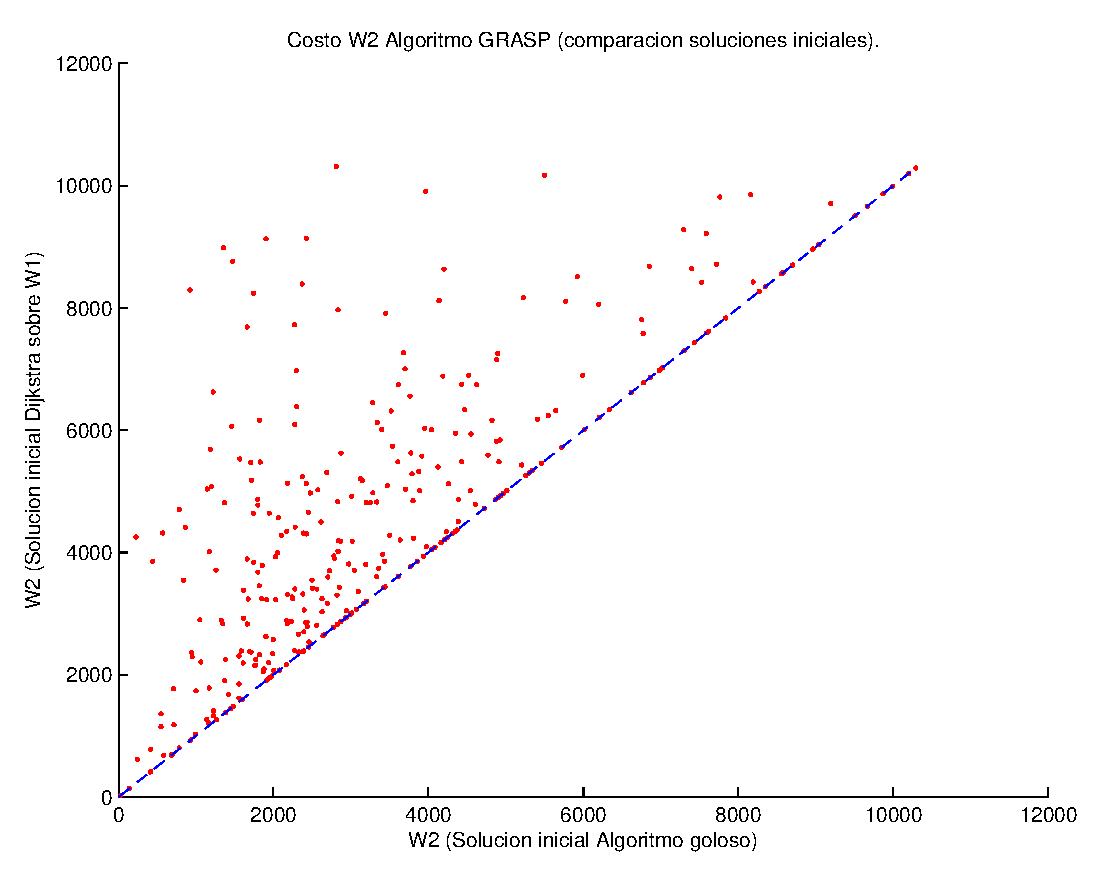
\includegraphics[width=\linewidth]{graficos/grasp_comparacion_soluciones_iniciales.eps}
      \caption{Comparación Soluciones iniciales}\label{fig:grasp-proporcion}
    \end{minipage}
  \end{center}
\end{figure}

Como podemos observar en el gráfico, frente a casos al azar, utilizar como solución inicial nuestro algoritmo goloso es mejor o igual que utilizar Dijkstra sobre $\omega_1$. Para facilitar la lectura, imprimimos una línea azul que representa a la función identidad.

Como utilizar nuestro algoritmo goloso como solución inicial nos devuelve los mejores resultados, decidimos utilizarla al momento de comparar las distintas heurísticas.